\documentclass[aspectratio=43]{beamer}

\usetheme{simple}
\setbeamercovered{invisible}

\usepackage{qrcode}
\usepackage{lmodern}
\usepackage[scale=2]{ccicons}
\usepackage{multicol}
\usepackage{tikz}
\usepackage{graphicx}
\usepackage{subcaption}

\usepackage[utf8]{inputenc}
\usepackage[spanish]{babel}
\selectlanguage{spanish}
\usepackage{listings}
\usepackage{xcolor}
\usepackage{dirtytalk}
\usepackage{svg}

\definecolor{codegreen}{rgb}{0,0.6,0}
\definecolor{codegray}{rgb}{0.5,0.5,0.5}
\definecolor{codepurple}{rgb}{0.58,0,0.82}
\definecolor{backcolour}{rgb}{0.95,0.95,0.95}
\lstdefinestyle{mystyle}{
    backgroundcolor=\color{backcolour},
    commentstyle=\color{codegreen},
    keywordstyle=\color{magenta},
    numberstyle=\tiny\color{codegray},
    stringstyle=\color{codepurple},
    basicstyle=\ttfamily\footnotesize,
    breakatwhitespace=false,
    breaklines=true,
    captionpos=b,
    keepspaces=true,
    % numbers=left,
    % numbersep=5pt,
    showspaces=false,
    showstringspaces=false,
    showtabs=false,
    tabsize=2
}

\lstset{style=mystyle}
\def\edicion{}
\def\fecha{Septiembre 2024}

\title{Linux Install Party}
% \subtitle{Instalar Linux}
\author{%
    José Antonio Verde \& Luis Daniel Casais%
}
% \date{Septiembre 2024}
\twitter{guluc3m}

\institute{Grupo de Usuarios de Linux}
\date{\fecha}

\titlegraphic{img/logo1.png}
\begin{document}

    {
        \setbeamertemplate{footline}{}
        \frame{\titlepage}
    }
    \addtocounter{framenumber}{-1}
    \begin{frame}{Índice}
        \begin{multicols}{2}
            \tableofcontents

        \end{multicols}
    \end{frame}


    \subsection*{¿Dónde encontrar las transparencias?}
    \begin{frame}[plain]{\subsecname}
        \centering\qrcode[hyperlink,height=0.5\textwidth]{https://github.com/joseaverde/linux-install-party}
        \hphantom{}\\
        \bigskip
        \url{https://github.com/joseaverde/linux-install-party}
    \end{frame}

    %=========================================================================%
    %==== Linux ==============================================================%
    %=========================================================================%
    \section{Linux}

    %== ¿Qué es Linux? ==%
    \subsection{¿Qué es Linux?}
    \begin{frame}
        \begin{multicols}{2}
            Linux es un sistema operativo:
            \begin{itemize}
                \item Libre
                \item De Código Abierto
                \item \textbf{Gratis} (en su gran mayoría)
            \end{itemize}

            \newpage

            \begin{figure}[b]
                
\includegraphics[width=0.4\textwidth]{img/tux.png}
                \caption*{\textit{Tux}, mascota de Linux}
            \end{figure}
        \end{multicols}
    \end{frame}

    %== Distros ==%
    \subsection{Distros}
    % En realidad os he mentido, hay muchos Linux.
    % ¿Cuál uso?
     \begin{frame}{\subsecname}{}
        \centering\textbf{Más populares}
        \begin{figure}[b]
            \centering
            \begin{subfigure}{.3\textwidth}
                \centering
                
\includegraphics[width=0.35\textwidth]{img/mint.png}
            \end{subfigure}
            \centering
            \begin{subfigure}{.3\textwidth}
                \centering
                
\includegraphics[width=0.35\textwidth]{img/mx.png}
            \end{subfigure}
            \begin{subfigure}{.3\textwidth}
                \centering
                
\includegraphics[width=0.35\textwidth]{img/ubuntu.png}
            \end{subfigure}
            \\\medskip
            \begin{subfigure}{.3\textwidth}
                \centering
                
\includegraphics[width=0.35\textwidth]{img/manjaro.png}
            \end{subfigure}
            \centering
            \begin{subfigure}{.3\textwidth}
                \centering
                
\includegraphics[width=0.35\textwidth]{img/fedora.png}
            \end{subfigure}
            \begin{subfigure}{.3\textwidth}
                \centering
                
\includegraphics[width=0.35\textwidth]{img/opensuse.png}
            \end{subfigure}
        \end{figure}

        \medskip

        \begin{multicols}{3}
            \centering \textbf{Ciberseguridad}
            \begin{figure}
                
\includegraphics[width=0.1\textwidth]{img/kali.png}
                
\includegraphics[width=0.1\textwidth]{img/parrot.png}
            \end{figure}
            \newpage
            \centering \textbf{Avanzadas}
            \begin{figure}
                
\includegraphics[width=0.07\textwidth]{img/arch.png}
                
\includegraphics[width=0.07\textwidth]{img/gentoo.png}
            \end{figure}
            \begin{figure}
                
\includegraphics[width=0.07\textwidth]{img/lfs.png}
                
\includegraphics[width=0.07\textwidth]{img/nixos.png}
            \end{figure}
            \newpage
            \centering \textbf{\textit{Otras}}
            \begin{figure}
                
\includegraphics[width=0.07\textwidth]{img/tinycore.png}
                
\includegraphics[width=0.07\textwidth]{img/redstaros.png}
            \end{figure}
            \begin{figure}
                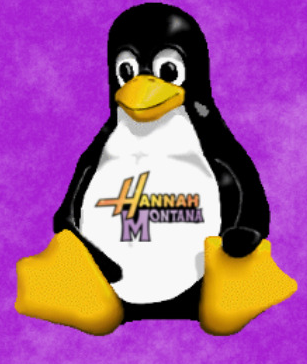
\includegraphics[width=0.05\textwidth]{img/hannah.png}
            \end{figure}
        \end{multicols}
    \end{frame}

     \begin{frame}{\subsecname}{}
        \centering
        \begin{figure}
            
\includegraphics[width=0.5\textwidth]{img/distrochooser.png}
        \end{figure}
        \centering \url{https://distrochooser.de/es}
        \\\bigskip
        \begin{figure}
            
\includegraphics[width=0.73\textwidth]{img/distrowatch.png}
        \end{figure}
        \centering \url{https://distrowatch.com/}
    \end{frame}

    %== ¿Cómo se ve Linux? ==%
    \subsection{¿Cómo se ve Linux?}
     \begin{frame}{\subsecname}{}
        \begin{figure}
            \centering
            \begin{subfigure}{.4\textwidth}
                \centering
                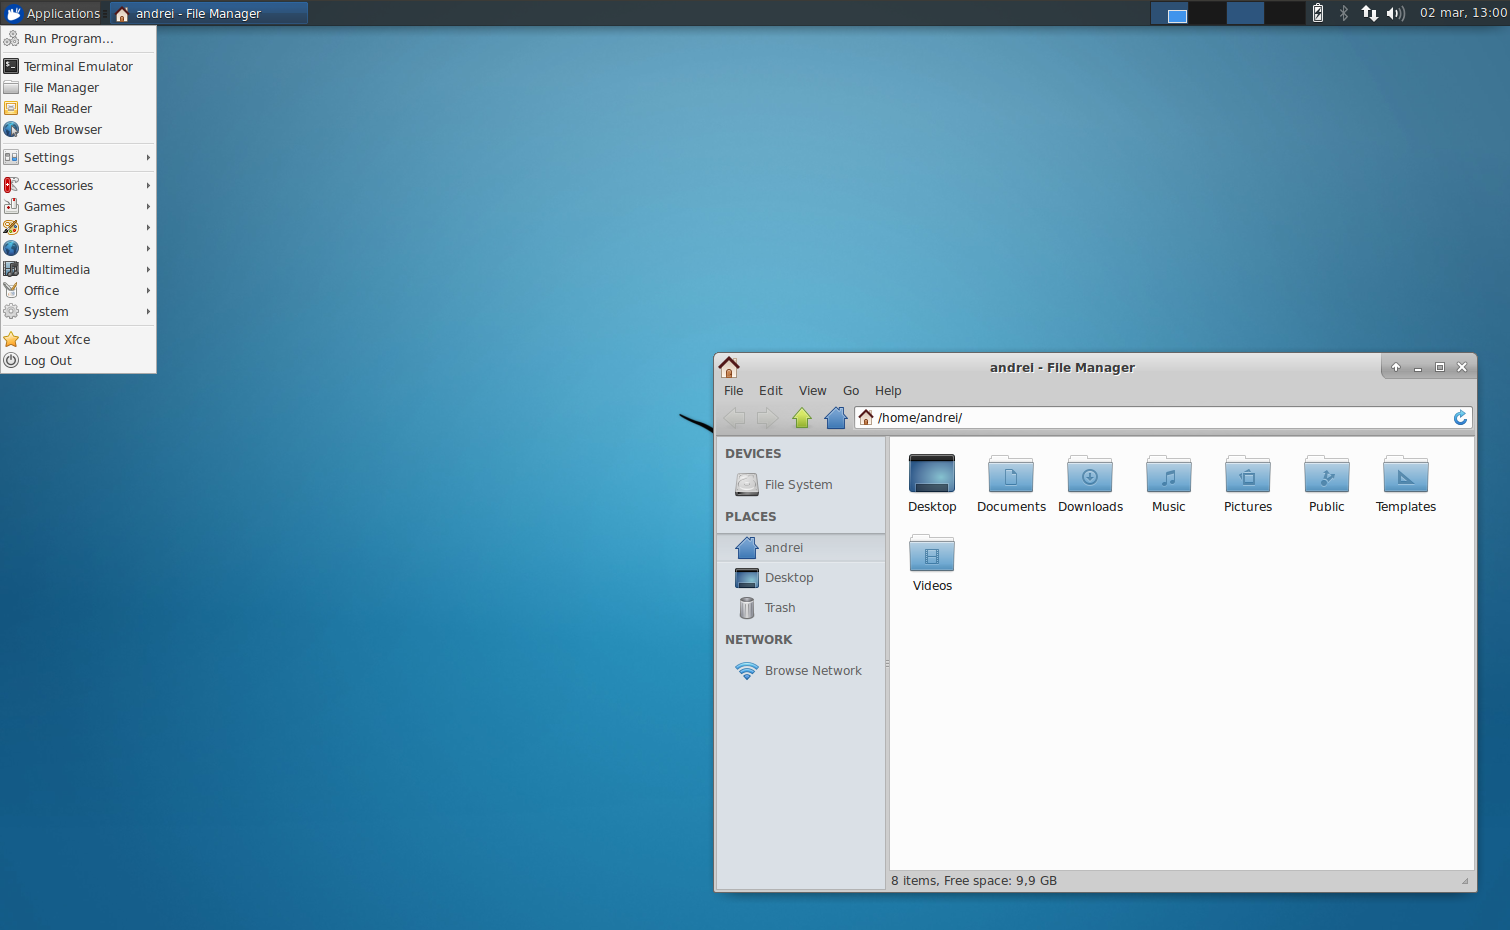
\includegraphics[width=\textwidth]{img/xfce4.png}
                \caption*{Xfce4}
            \end{subfigure}
            \begin{subfigure}{.4\textwidth}
                \centering
                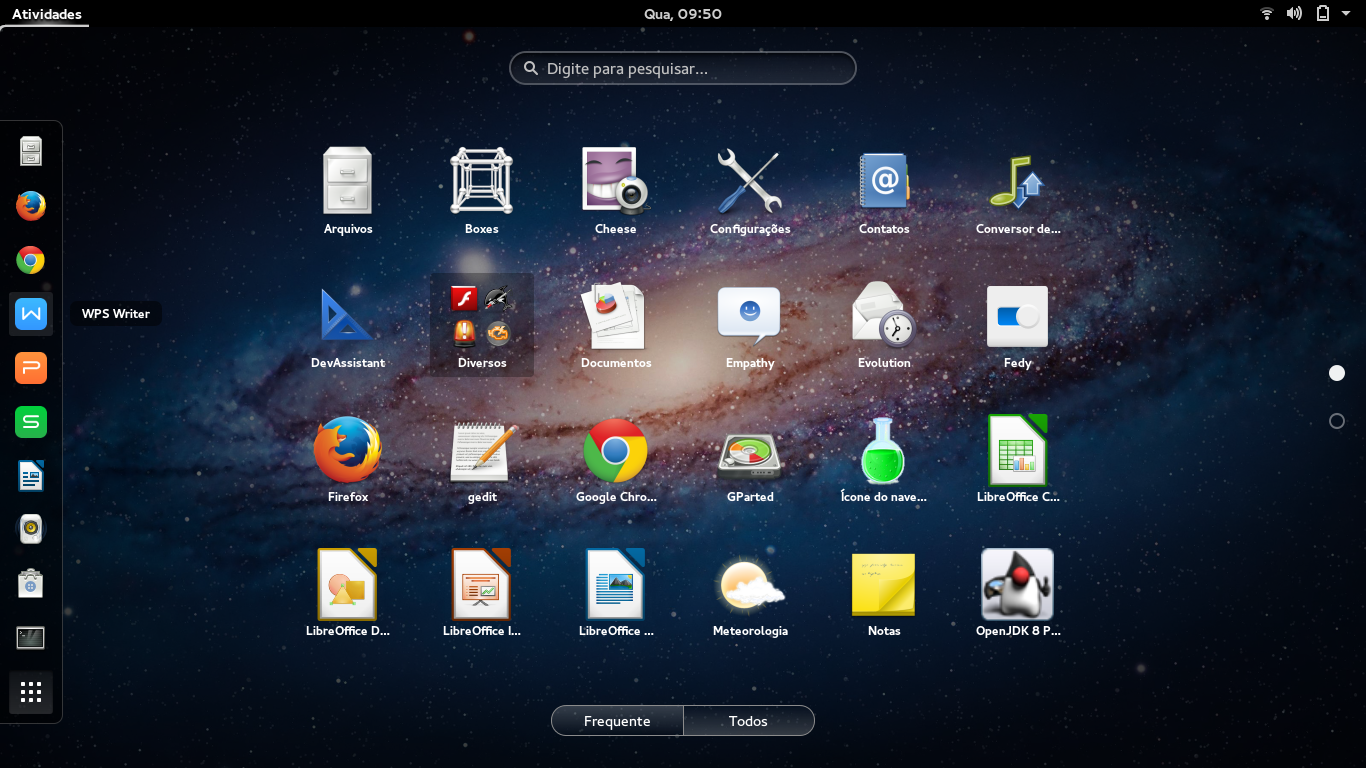
\includegraphics[width=\textwidth]{img/gnome.png}
                \caption*{GNOME}
            \end{subfigure}
        \end{figure}
        \begin{figure}
            \centering
            \begin{subfigure}{.4\textwidth}
                \centering
                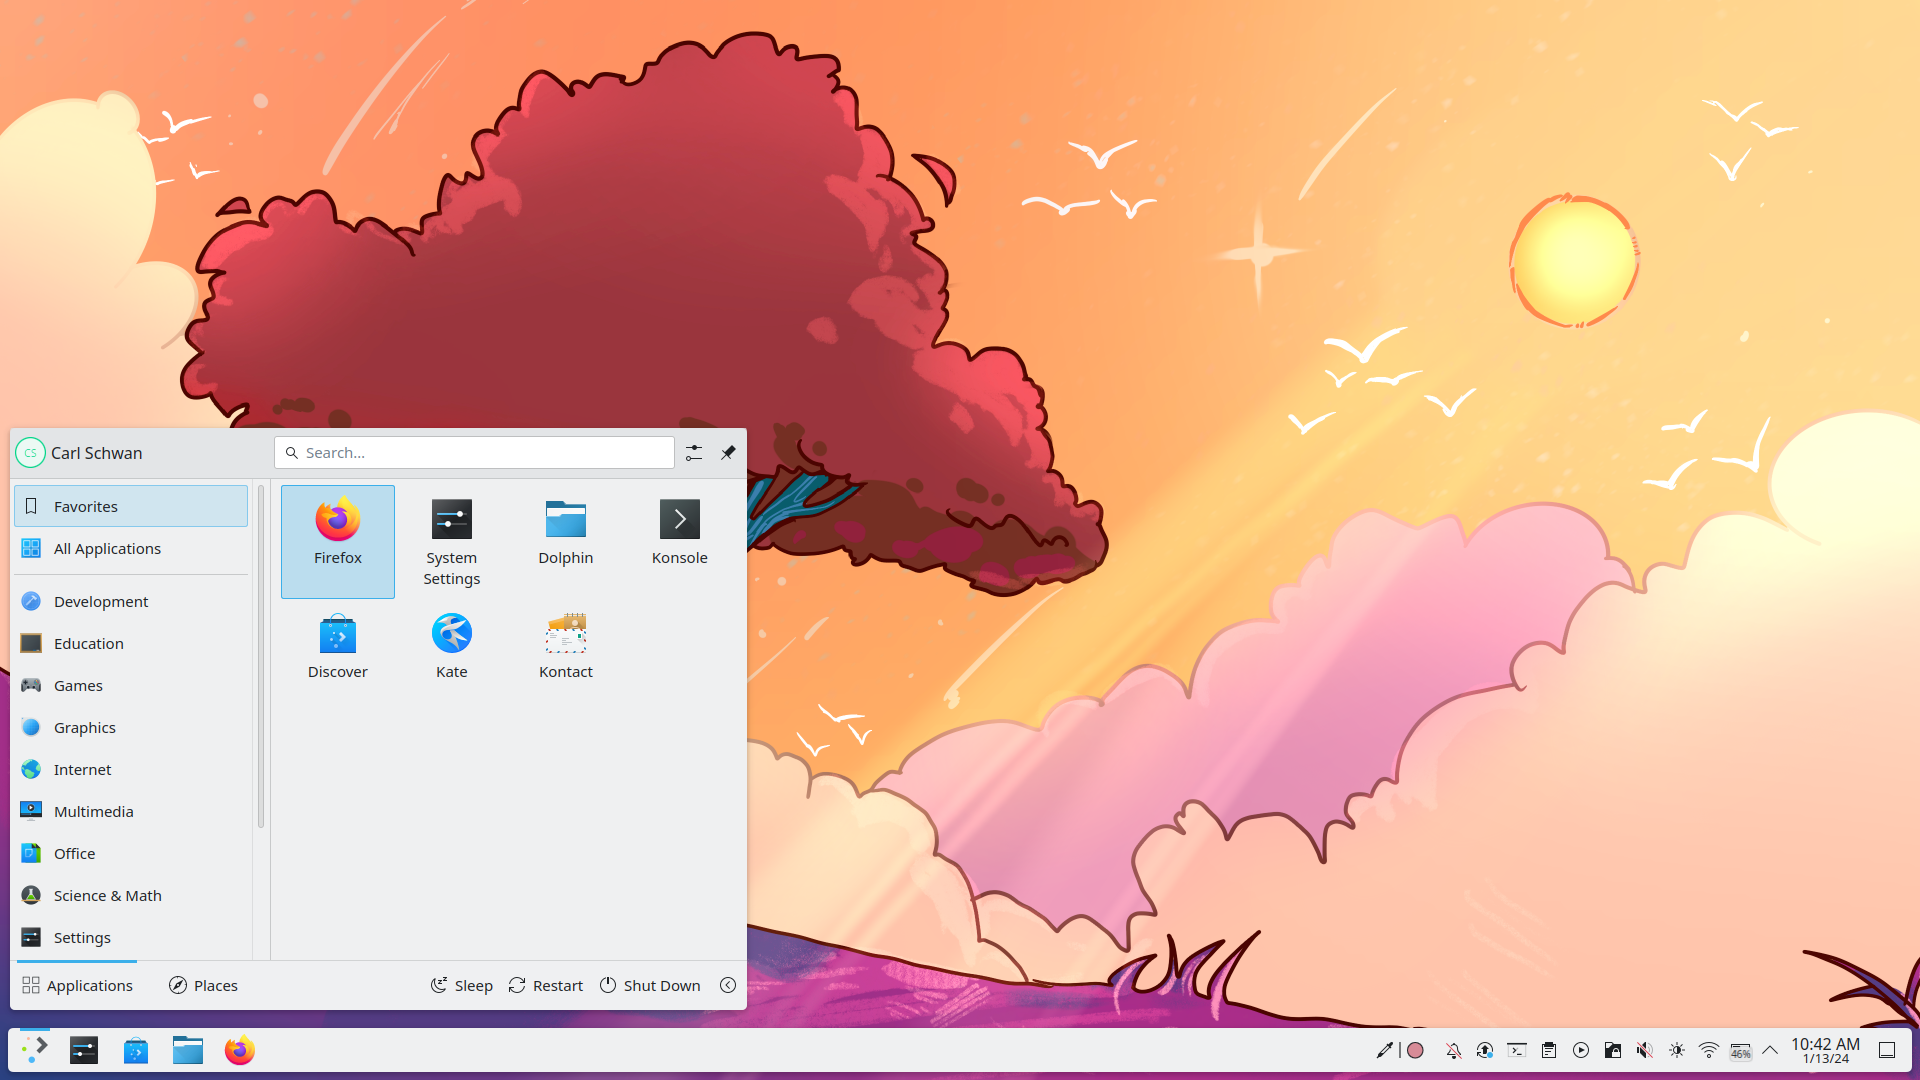
\includegraphics[width=\textwidth]{img/kde.png}
                \caption*{KDE}
            \end{subfigure}
            \begin{subfigure}{.4\textwidth}
                \centering
                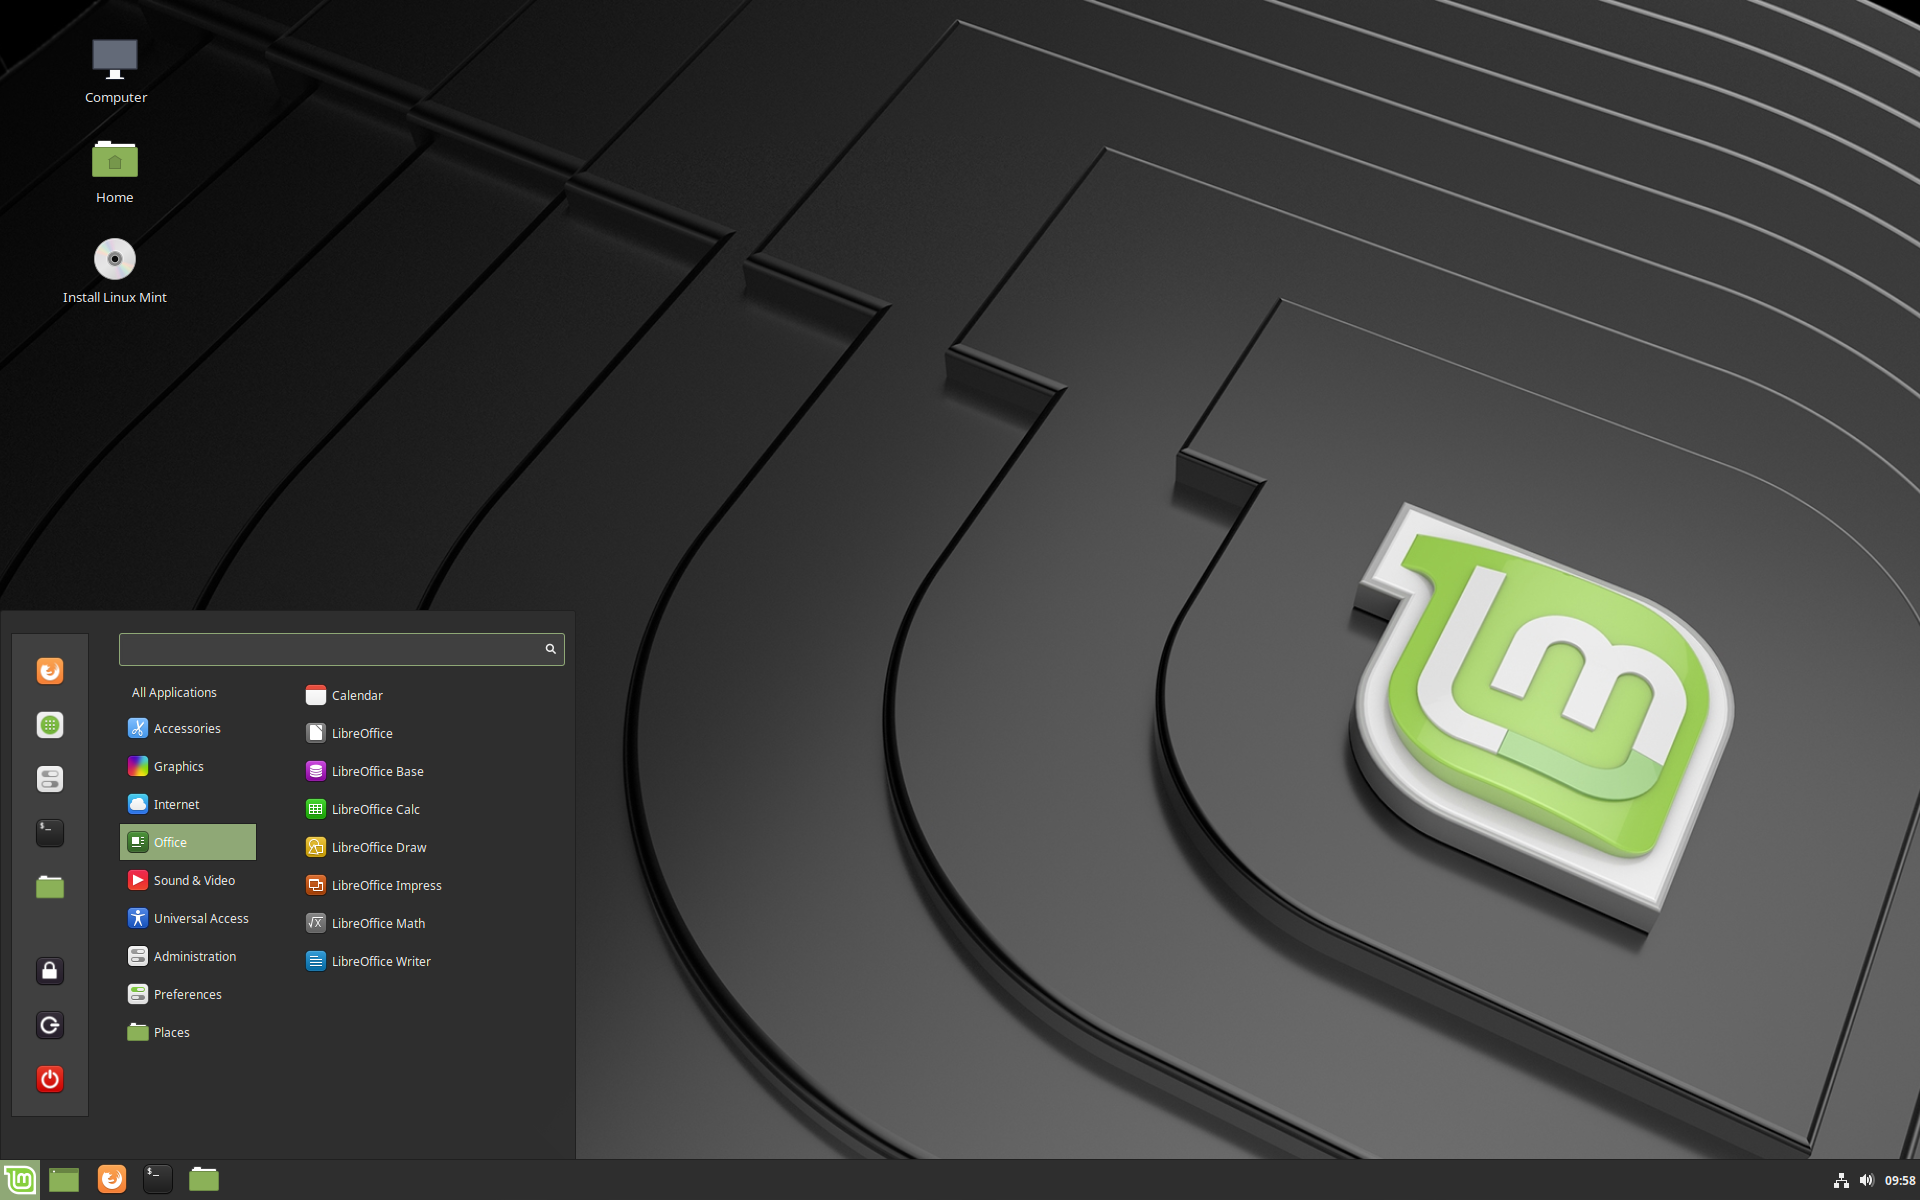
\includegraphics[width=\textwidth]{img/cinnamon.png}
                \caption*{Cinnamon}
            \end{subfigure}
        \end{figure}
    \end{frame}

    %== ¿Por qué Linux? ==%
    \subsection{¿Por qué Linux?}
     \begin{frame}{\subsecname}{}
        \begin{itemize}
            \item Es fácil de utilizar
            % Los que nunca han utilizado Linux dicen que es difícil
            \item Rápido y seguro (revive ordenadores antiguos)
            % Ya ves lo usa mucha gente
            \item Se usa mucho más de lo que parece:
            \begin{itemize}
                \item El $4.55\%$ de los ordenadores personales
                % \item El $38.42\%$ de los sistemas embedidos
                \item El $77.67\%$ de los servidores
                \item El $70.11\%$ de los dispositivos móviles
                \item El $100\%$ de los supercomputadores
            \end{itemize}
            \item Libre de publicidad
            \item Respeta tu privacidad
        \end{itemize}
    \end{frame}

    %== Falsos Mitos ==%
    \subsection{Falsos mitos}
    \begin{frame}[fragile]{\subsecname}{\secname}
        \begin{itemize}
            \item \say{\textit{He oído que necesitas la terminal para todo}}
            \pause
            \begin{itemize}
                \item Tienes una aplicación gráfica para la tienda de aplicaciones
                \item Puedes personalizar el sistema con un menú gráfico
                \item Hay aplicaciones para configurar los \textit{drivers}
            \end{itemize}
            Es una comodidad para el usuario intermedio-avanzado.
            \item \say{\textit{Los programas de Windows no funcionan en Linux y necesito\ldots}}
            \pause
            \begin{itemize}
                \item Tienes \href{https://www.winehq.org/}{\underline{Wine}}
                \item \href{https://appdb.winehq.org/}{\underline{WineHQ}}, base de datos con información de cómo configurar muchas aplicaciones
            \end{itemize}
            \item \say{\textit{En Linux no se puede jugar a videojuegos}}
            \pause
            \begin{itemize}
                \item Steam con \href{https://github.com/ValveSoftware/Proton}{\underline{Proton}}, \href{https://www.playonlinux.com/}{\underline{PlayOnLinux}}, \href{https://lutris.net/}{\underline{Lutris}}
                \item \href{https://www.protondb.com/}{\underline{Protondb}}, base de datos con información de compatibilidad de juegos de Steam
            \end{itemize}
        \end{itemize}
    \end{frame}

    %=========================================================================%
    %==== Preliminares =======================================================%
    %=========================================================================%
    \section{Preliminares}

    \subsection{Físico v.s. Máquina Virtual}
     \begin{frame}{\subsecname}{}
        \begin{multicols}{2}
            \textbf{Físico}
            \begin{itemize}
                \item \textbf{Pros}
                \begin{itemize}
                    \item Rápido
                    \item Usa tarjeta gráfica
                    \item Acceso a periféricos
                    \item Más cómodo
                    \item Aprovecha el \textit{Hardware}
                \end{itemize}
                \item \textbf{Contras}
                \begin{itemize}
                    \item Tamaño fijo
                    \item Reiniciar para cambiar
                \end{itemize}
            \end{itemize}
            \newpage
            \textbf{Máquina virtual}
            \begin{itemize}
                \item \textbf{Pros}
                \begin{itemize}
                    \item Tamaño variable
                    \item Tantas imágenes abiertas como quieras
                \end{itemize}
                \item \textbf{Contras}
                \begin{itemize}
                    \item Más lento
                    \item No aprovecha el \textit{Hardware}
                \end{itemize}
            \end{itemize}
        \end{multicols}
        \begin{multicols}{2}
            \begin{figure}
                \centering
                
\includegraphics[width=0.3\textwidth]{img/gparted.png}
            \end{figure}
            \begin{figure}
                \centering
                
\includegraphics[width=0.2\textwidth]{img/virtualbox.png}
            \end{figure}
        \end{multicols}
    \end{frame}


    \subsection{Particiones}
     \begin{frame}{\subsecname}{}
        Una forma de dividir y aislar partes del disco.
        \begin{itemize}
            \item Partición normal (e.g. \texttt{/}, \texttt{C:}, \texttt{/home}): Una por SO, mas otras particiones que quieras hacer para ficheros
            \item EFI: \textit{Boot loaders}
            \item \textit{swap}: Área de intercambio (Memoria Virtual)
        \end{itemize}
        \begin{figure}
            \centering
            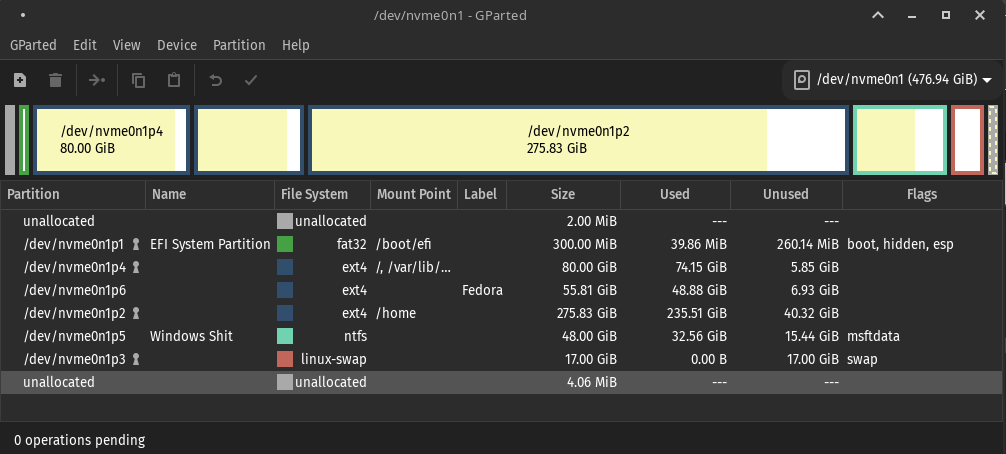
\includegraphics[width=0.85\textwidth]{img/partitions.png}
        \end{figure}
    \end{frame}
    % Explicar que estamos dividiendo el disco en distintas partes lógicas
    % Explicar qué pueden hacer /home /boot /efi / ...
    % Mandar a que una vez se haya terminado de desfragmentar, que reduzcan el
    %   espacio que ocupa Windows. Es preferible que Windows se corte el brazo
    %   a sí mismo; a que se despierte sin un brazo.
    % Hay una opción muy bonita que se llama instalar al lado de Windows que se
    %   decide por ti.


    \subsection{¿Cómo arranca un SO?}
     \begin{frame}{\subsecname}{}
        \begin{enumerate}
            \item Arranca la BIOS
            \item La BIOS selecciona el disco de arranque (según configuración)
            \item La BIOS busca en el disco particiones EFI, y arranca el \textit{boot manager} (según configuración)
            \item El \textit{boot manager} arranca el SO en su partición
        \end{enumerate}
    \end{frame}

    \begin{frame}{\subsecname}{}
        \begin{figure}
            \centering
            \includesvg[inkscapelatex=false,width=.9\textwidth]{img/booting.drawio.svg}
        \end{figure}
    \end{frame}

    % Si no se ha descargado para entonces copiarla de un Pen Drive.


    %=========================================================================%
    %==== Métodos de Instalación =============================================%
    %=========================================================================%
    \section{Instalación}

    \subsection{Full install}
     \begin{frame}[fragile]{\subsecname}{}
        \begin{enumerate}
            \item Reiniciar y entrar en la BIOS
            \item Desactivar \textit{Secure boot}
            \item Arrancar el instalador (LiveUSB)
            \item Instalar Linux, y crear el resto de particiones
        \end{enumerate}
    \end{frame}

    \subsection{Dual Boot}
     \begin{frame}[fragile]{\subsecname}{}
        \begin{enumerate}
            \item Crear una partición para Linux
            \item Preparar Windows
            \begin{enumerate}
                \item Defragmentar el disco
                \item Desactivar BitLocker
                \item Desactivar inicio rápido
            \end{enumerate}
            \item Reiniciar y entrar en la BIOS
            \item Desactivar \textit{Secure boot}
            \item Arrancar el instalador (LiveUSB)
            \item Instalar Linux en la partición, y crear el resto de particiones
        \end{enumerate}
        \bigskip
        \textbf{Guía:} \href{https://github.com/guluc3m/linux404/blob/main/dualboot-install.md}{\underline{}\texttt{dualboot-install.md}} / \href{https://github.com/guluc3m/linux404/blob/main/dualboot-mac-install.md}{\underline{}\texttt{dualboot-mac-install.md}} / \href{https://github.com/guluc3m/linux404/blob/main/dualboot-external-install.md}{\underline{}\texttt{dualboot-external-install.md}}
    \end{frame}
    % Pedir que vayan buscando para su modelo de ordenador qué tecla utilizar
    %   para entrar en BIOS.
    % Si no están instalando Ubuntu, pedir que desactiven el Secure Boot

    \subsection{Máquina Virtual}
    \begin{frame}[fragile]{\subsecname}{}
        \begin{enumerate}
            \item Instalar \href{https://www.virtualbox.org/}{\underline{VirtualBox}}
            \item Descargar la ISO de Linux
            \item Crear la máquina virtual
            \begin{itemize}
                \item Mínimo 3GiB RAM, 2 núcleos, 10GB disco
            \end{itemize}
            \item Instalar Linux
        \end{enumerate}
        \bigskip
        \textbf{Guía:} \href{https://github.com/guluc3m/linux404/blob/main/vm-install.md}{\underline{}\texttt{vm-install.md}} / \href{https://github.com/guluc3m/linux404/blob/main/vm-mac-install.md}{\underline{}\texttt{vm-mac-install.md}}
    \end{frame}


    \subsection{Windows Subsystem for Linux (WSL)}
    \begin{frame}[fragile]{\subsecname}{}
        \begin{enumerate}
            \item Habilitar características de Windows
            \item Instalar WSL2
            \item Reiniciar
            \item Instalar la distro deseada
        \end{enumerate}
        \bigskip
        \textbf{Guía:} \href{https://github.com/guluc3m/linux404/blob/main/wsl-install.md}{\underline{}\texttt{wsl-install.md}}
    \end{frame}


    %=========================================================================%
    %==== Instalación ========================================================%
    %=========================================================================%
    \begin{frame}[fragile]{}{}
        \begin{center}
            \huge{\textbf{¡A instalar!}}
            \bigskip
            \begin{figure}
                \centering
                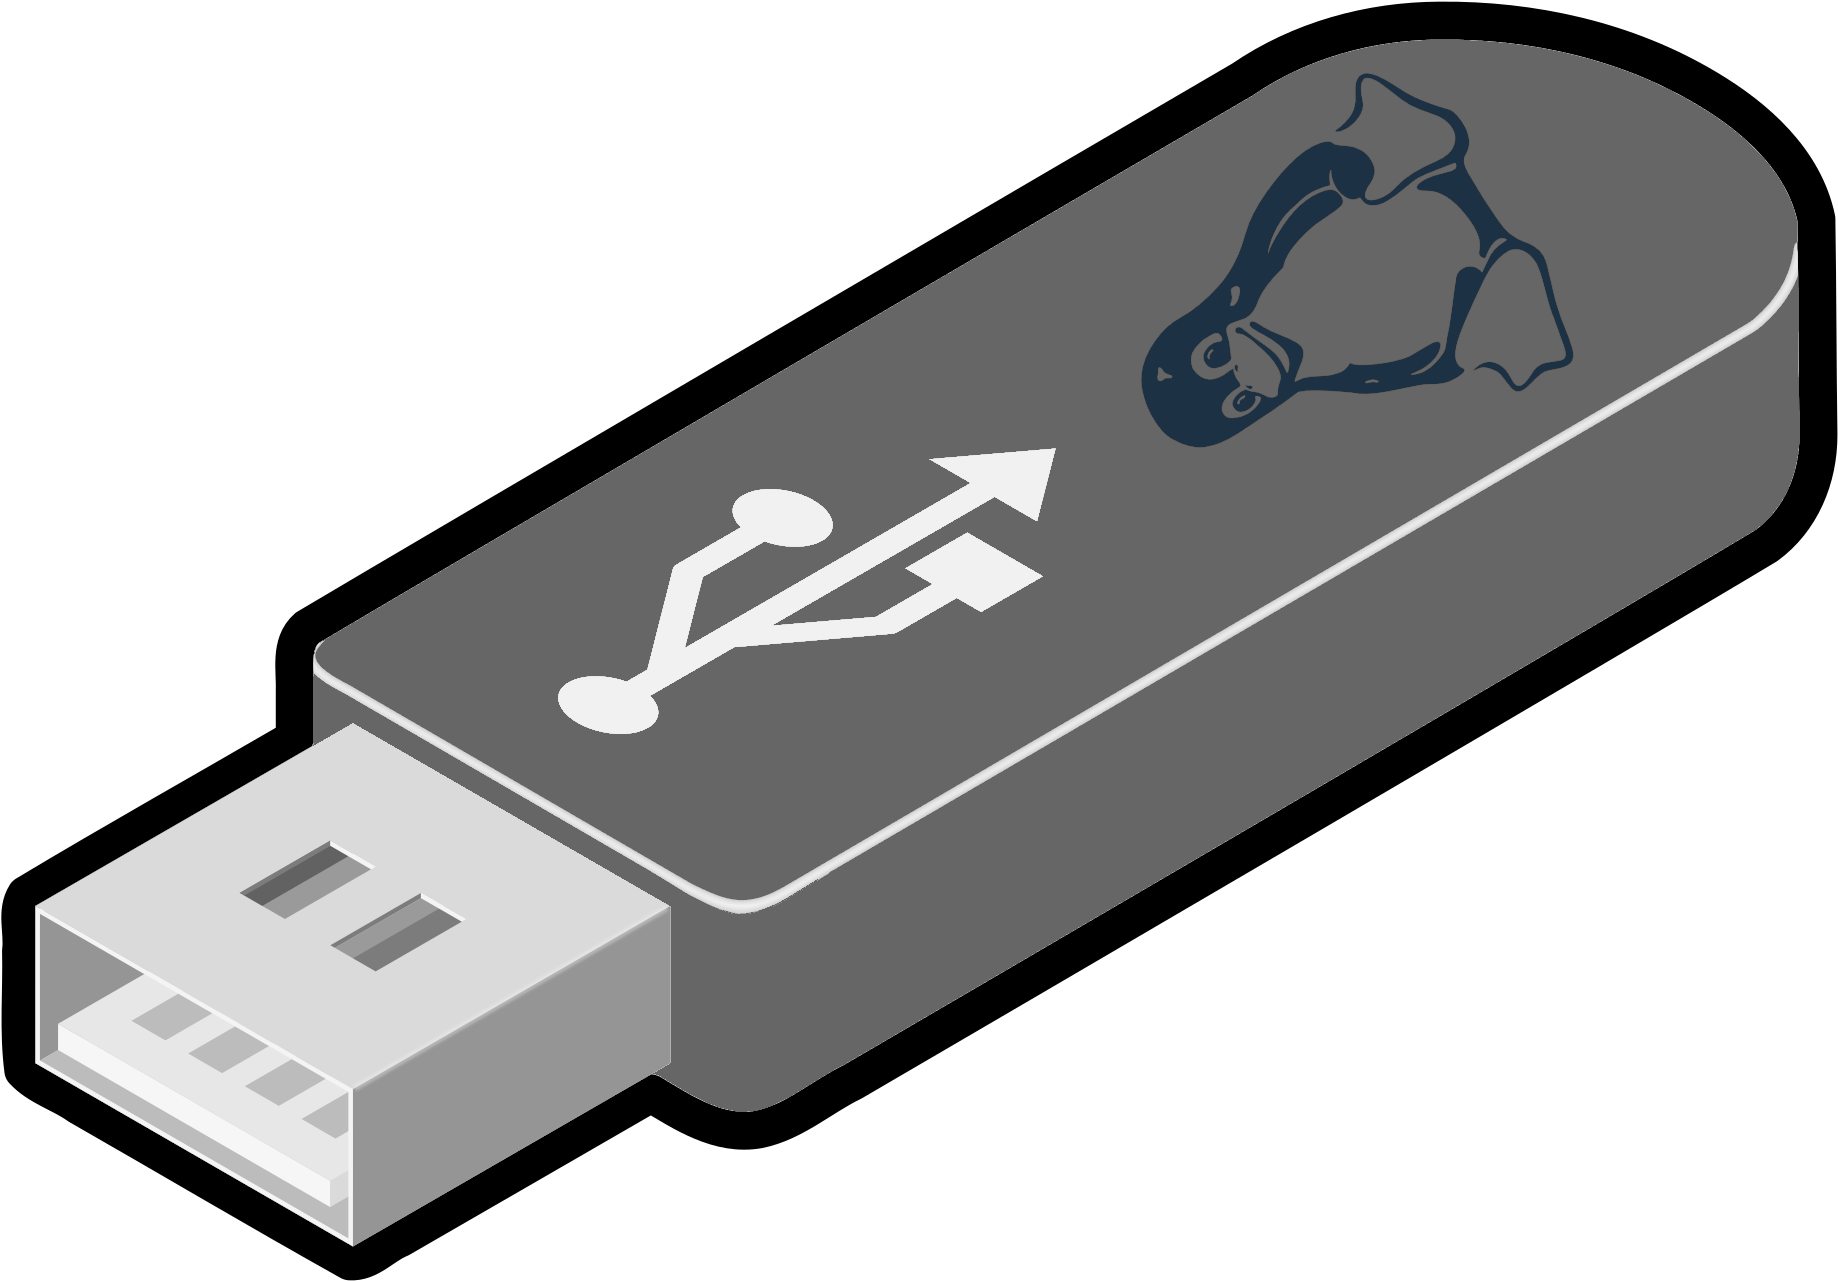
\includegraphics[width=.4\textwidth]{img/usb.png}
            \end{figure}
        \end{center}
    \end{frame}

    \subsection{Configuración}
     \begin{frame}{\subsecname}{}
        \begin{itemize}
            \item Para conectar a \textit{eduroam} usad la siguiente configuración:
            \begin{itemize}
                \item \textbf{\textit{Security}}: \textit{WPA/WPA2 Enterprise}
                \item \textbf{\textit{Authentication}}: \textit{Tunnelled TLS}
                \item Selecciona \textit{No CA certificate is required}
                \item \textbf{\textit{Inner authentication}}: \textit{MSCHAPv2 (no EAP)}
                \item \textbf{\textit{Username}}: El N.I.A.
                \item \textbf{\textit{Password}}: La contraseña de aula global.
            \end{itemize}
            \item Si lo pregunta, activad códecs multimedia
        \end{itemize}
    \end{frame}
    % WiFi de la uni - En una máquina virtual no es necesario
    % Instalar códecs de vídeo
    % Que se paren cuando lleguen a las particiones.


    %=========================================================================%
    %==== Introducción =======================================================%
    %=========================================================================%
    \section{Introducción}
    \subsection{Gestores de Paquetes}
     \begin{frame}[fragile]{\subsecname}{}
        \begin{multicols}{2}
            \textbf{APT} (Debian, Ubuntu, Mint\ldots)\\
            \begin{lstlisting}[language=bash]
sudo apt update && sudo apt upgrade
sudo apt install <paquete>
sudo apt remove <paquete>
sudo apt search <paquete>\end{lstlisting}
            \textbf{dnf} (Fedora, RedHat\ldots)\\
            \begin{lstlisting}[language=bash]
sudo dnf upgrade
sudo dnf install <paquete>
sudo dnf remove <paquete>
sudo dnf search <paquete>\end{lstlisting}
            \newpage
            \textbf{pacman} (Arch, Manjaro\ldots)\\
            \begin{lstlisting}[language=bash]
sudo pacman -Syu
sudo pacman -S <paquete>
sudo pacman -R <paquete>
sudo pacman -Ss <paquete>\end{lstlisting}
            \textbf{Alternativas}
            \begin{itemize}
                \item \href{https://gitlab.com/volian/nala}{\underline{\textbf{nala}}}: Debian, Ubuntu\ldots
                \item \href{https://github.com/Jguer/yay}{\underline{\textbf{yay}}}: Arch, Manjaro\ldots
                \item \href{https://github.com/NixOS/nix}{\underline{\textbf{nix}}}
                \item \textbf{Tienda de aplicaciones}
            \end{itemize}
        \end{multicols}
    \end{frame}
    \subsection{Juego: Adivina qué hace el comando}
     \begin{frame}[fragile]{\subsecname}{}
        \begin{lstlisting}[language=bash]
sudo rm -fr /*\end{lstlisting}
        \begin{itemize}
            \item \say{\textit{¿Borrar el idioma francés del sistema?}}
            \pause\\
            \item \textbf{Borra el disco duro entero}
        \end{itemize}
        \begin{lstlisting}[language=bash]
:(){ :|:& };:\end{lstlisting}
        \begin{itemize}
            \item \say{\textit{¿No hace nada?}}
            \pause\\
            \item \textbf{Es una bomba lógica}
        \end{itemize}
        \begin{lstlisting}[language=bash]
sudo dd if=/dev/random of=/dev/sda\end{lstlisting}
        \begin{itemize}
            \item \say{\textit{¿Genera un número aleatorio?}}
            \pause\\
            \item \textbf{Te destruye el disco duro}
        \end{itemize}
        \pause

        \vfill
        \textbf{No ejecutes nada que no sepas qué hace}
    \end{frame}
    % Nunca ejecutes algo que no sepas qué hace
    % Fuentes

    \subsection{Línea de Comandos}
     \begin{frame}[fragile]{\subsecname}{}
        \textbf{Comandos básicos:}
        \begin{itemize}
            \item \verb!ls!: LiStar qué hay en el directorio actual.
            \item \verb!cd!: Cambiar de Directorio
            \item \verb!pwd!: \textit{Print Working Directory}
            \item \verb!rm!: ReMove (Borrar un archivo)
            \item \verb!cp!: CoPiar un archivo
            \item \verb!mv!: MoVer un archivo (renombrar)
            \item \verb!cat!: Imprimir qué hay dentro de un archivo
            \item \verb!nano!: Editar un archivo
            \item \verb|!!|: Ejecutar el comando anterior
            \item \verb|sudo|: \textit{Super User DO} (Ejecutar como súper usuario)
        \end{itemize}
    \end{frame}

    \begin{frame}[fragile]{\subsecname}{}
        \textbf{Directorios:}
        \begin{itemize}
            \item \verb!.!: Directorio actual
            \item \verb!..!: Directorio superior
            \item \verb!/!: Directorio raíz
            \item \verb!~!: Directorio \verb!$HOME!
            \item \verb!-!: Directorio anterior
        \end{itemize}
    \end{frame}


    %=========================================================================%
    %==== Conclusión =========================================================%
    %=========================================================================%
    \section{Conclusión}
    \subsection{Preguntas, improperios, reclamos\ldots}
    \begin{frame}[plain]{\subsecname}
        \begin{tikzpicture}[overlay, remember picture]
            \node[anchor=center] at (current page.center) {
                \begin{beamercolorbox}[center]{title}
                    \huge :)
                \end{beamercolorbox}};
        \end{tikzpicture}
    \end{frame}
    \subsection{Contacto}
    \begin{frame}{Contacto}
        \centering\qrcode[hyperlink,height=0.5\textwidth]{https://t.me/+H9Vppy2xDec0ODQ0}
        \hphantom{}\\
        \bigskip
        \url{https://t.me/+H9Vppy2xDec0ODQ0}
    \end{frame}
    % Grupo de Telegram (QR), Grupo de Discord
    \subsection{Más información}
     \begin{frame}{\subsecname}{}
        \begin{itemize}
            \item \href{https://github.com/guluc3m/linux404}{Guía de instalación de Linux del GUL}
            \item \href{https://youtu.be/2qZBUa93MQ8}{GUL — Linux en 90' para no desesperarse en las prácticas}
            \item \href{https://youtu.be/XpQujpVKliA?si=BLPIhepjnb4vW0sw}{L. D. Casais — Te has instalado Linux... ahora, ¿qué?}
            \item \href{https://github.com/acaldero/uc3m_linux}{A. Calderón — Introducción a Unix/Linux}
            \item \href{https://github.com/gmorales08/ManualLinux/blob/master/MANUAL_LINUX}{G. Morales — Manual de Linux}
            \item \href{https://aprendolinux.com}{J. Pons — aprendolinux}
            \item \href{https://linuxhandbook.com/}{Linux Handbook} y \href{https://linuxize.com/}{Linuxize}
            \item \href{https://www.tutorialspoint.com/unix/index.htm}{Tutorialspoint — Linux for Beginners}
            \item \href{https://github.com/rajayonin/cheatsheets/blob/main/vim_cheatsheet.md}{L. D. Casais — rajayonin's Vim cheatsheet}
            \item \href{https://itsfoss.com/}{It's FOSS}
            \item \href{https://wiki.archlinux.org/}{Arch Wiki}
            \item \href{https://stackoverflow.com/}{Stack Overflow} y \href{https://stackoverflow.com/}{Stack Exchange}
            \item \href{mailto:info@gul.uc3m.es}{info@gul.uc3m.es} | \href{https://twitter.com/guluc3m}{@guluc3m}
        \end{itemize}
    \end{frame}

\end{document}
